% !TeX spellcheck = en_US
% !TeX encoding = UTF-8
% !TeX root = ../document.tex

\chapter{Model Unspecific Search}

\section{Motivation}
A collision at an energy of \SI{13}{\TeV} can create a large amount of different particles. Solely by combinatorics, it follows that a lot of different final states are accessible.

Most dedicated searches tend to focus on one or a few final states that represent the signature of the theory under investigation. This leaves many final states not examined, either because of the complexity of the final state or because there is no analysis group currently working on a corresponding theory.

One of the goals of the model unspecific search is to gain knowledge from these additional final states. Additionally, the model unspecific search aims to obtain a global interpretation of the agreement between simulation and observed data across a broad range of final states.

\section{Previous Works}
The approach of a model unspecific search is not a new concept: In 1998, a note about an unspecific search has been written at the L3 experiment (\ac{LEP})\cite{Hebbeker:GlobalComparisonL3}, and in 2004, a similar approach has been applied to data of the D0-experiment at the Tevatron proton-antiproton collider at Fermilab\cite{Biallass:ModelIndependentSearch}.

At \ac{CMS}, the analysis has been developed and regularly applied to observed data since 2009\cite{Schmitz:ModelUnspecificSearch,Hof:ImplementationModelIndependent,Dietz-Laursonn:ModelUnspecificSearch,Olschewski:StudyAlternativeStatistical,Brodski:ModelUnspecificSearch,Pieta:MUSiCModelUnspecific,Papacz:ModelUnspecificSearch,Albert:ExtensionModelUnspecific,Roemer:ModelUnspecificSearch,CMS:CMS-PAS-EXO-14-016,Knutzen:softwarereinterpretationmodel,Durchardt:MUSiCModelUnspecific}. 
This thesis bases on the most recent implementation of the \ac{MUSiC} analysis.\todo{ok so?}

Very recently, the \ac{ATLAS} collaboration published a conference note analyzing \SI{3.2}{\per\femto\barn} of \ac{LHC} data at $\sqrt{s} = \SI{13}{\TeV}$ using a similar model-independent search \cite{ATLAS:ATLAS-CONF-2017-001}. 

\section{Procedure}
The input to the \ac{MUSiC} analysis are reconstructed events of observed as well as simulated data, which have been centrally reconstructed by the \ac{CMS} collaboration.
As first step of the \ac{MUSiC} analysis, requirements on events and physics objects are applied, discarding unwanted events and extracting objects for the \ac{MUSiC} analysis (see \fref{chap:selection}).
Afterwards, each event is classified sorted into so-called \emph{event classes}, sets of events that share the same final state.
For each event class, the kinematic variables of each event are calculated and \emph{kinematic distributions} are aggregated.
Up to this point, the same procedure is applied to simulated data and observed data.
Subsequently, an automated search algorithms finds the largest deviation between data and simulation within each kinematic distribution of each event class. Afterwards, the global significance of each deviation is estimated from Standard-Model only simulations.

\section{Transverse Momentum and Energy}
\label{sec:transverse_quantities}

As prerequisite for the following sections it is helpful to introduce the so-called transverse quantities \emph{transverse momentum} and \emph{transverse energy}. This section provides a motivation and definition for both.

Interaction cross sections are often dependent on the amount of momentum involved. In t-channel diagrams, the entire momentum transfer can be measured by calculating the combined invariant mass of decay products.
In order to achieve this goal, one must know all four components of the momentum of all created particles. If the final state contains neutrinos, which are not detectable by the detector, this is not achievable.

In other experiments like \ac{LEP}, one could use conservation of momentum and the known momentum of colliding particles to reconstruct the neutrino four-momentum and the momentum transfer. At the \ac{LHC} this is also impossible: The total proton momentum is distributed unevenly between the constituent quarks and gluons and thus the momentum involved in a collision is only known up to statistical probability.

The mitigation pursued at \ac{CMS} is to only regard kinematics in the transverse plane, orthogonally to the beam pipe. Projection of the kinematic (three-)momentum onto the transverse plane gives the transverse momentum \pT.

There are other properties of the transverse momentum that make it an interesting quantity: It can be straightforwardly measured from the tracks since the magnetic field lines are parallel to the beam direction and the Lorentz force only acts in the transverse plane. Additionally, the transverse momentum is not only invariant to the actual distribution of momenta within the proton, but also to Lorentz boosts along the $z$-axis. 

Assuming $p_x$, $p_y$, $E$ and $m$ can be observed directly (e.g. via track curvature) or indirectly (e.g. via particle identification), we can define the transverse momentum and transverse energy as follows:
\begin{align*}
\vec{p}_T &\defeq \left( p_x, p_y, 0 \right)^T  \\
\vec{E}_T &\defeq E \frac{\vec{p}_T}{\abs{\vec{p}}} = \frac{\vec{p}_T}{\sqrt{1-\left(m/E\right)^2}}
\end{align*}

Note that in the approximation of massless ($m \approx 0$) particles: $\vec{p}_T = \vec{E}_T$. % $ = \vec{M}_T$.


\section{Event Selection}
The following section will discuss how events are selected to be used for the \ac{MUSiC} analysis. This is tightly related to the section after, where concepts for the reconstruction of physics objects from recorded events are selected.

Since this thesis aims to be a general evaluation of the \ac{MUSiC} approach, we will not go deep into detail about the algorithms used, nor the exact parameter values. For the sensitivity studies in \fref{chap:sensitivity_studies}, however, specific values have to be chosen. If not explicitly stated otherwise, values of the 2015 analysis run are used and can be found in \cite{Roemer:ModelUnspecificSearch}.

\subsection{Triggers}
\newcommand{\trigger}[1]{\texttt{\detokenize{#1}}}
\Fref{sec:triggering} described the trigger, dedicated hardware that decides whether observed events are recorded to disk. In the vocabulary of an analyst, the term "trigger" does not only refer to the required hardware, but also to the set of rules that are applied. In practice, triggering hardware is configured to run multiple sets of rules in a so-called \emph{trigger menu}, as to maximize the usage of readout bandwidth without overloading the available resources.
The triggering decision is also simulated on \ac{MC} generated events: Using the same information available to the triggering system and a trigger emulator, each event is assigned tags about which decision lead to it being stored. 

Because multiple trigger configurations are running at the same time, the same event might end up in two separate trigger streams. In the analysis, one thus has to take care to remove events that are duplicated this way.
An additional problem arises in the first few \si{\GeV} beyond the \pT threshold: In this so-called \emph{turn-on} region, disagreement between observed data and simulation has been found which is accounted to insufficiencies in the simulation. Because of this, an additional minimum \pT threshold close above the trigger threshold is applied.

\Fref{tab:triggers} provides a reference of triggers used in the analysis. In comparison to the 2015 analysis, the \pT threshold of the single electron trigger has been raised from \SI{105}{\GeV} to \SI{115}{\TeV}. This choice ensures consistency between the 2015 and 2016 analysis for the sensitivity study.

\begin{table}
    \centering
    \begin{tabular}{l l l}
    \toprule
    Stream Name & trigger $p_\text{T, min}$ & custom $p_\text{T, min}$ \\
    \midrule
    \trigger{HLT_Ele115_CaloIdVT_GsfTrkIdT} & \SI{115}{\GeV} & \SI{120}{\GeV} \\
    \trigger{HLT_DoubleEle33_CaloIdL_GsfTrkIdVL_MW} & \SI{33}{\GeV}, \SI{33}{\GeV} & \SI{50}{\GeV}, \SI{50}{\GeV} \\
    \trigger{HLT_Mu50} & \SI{50}{\GeV} & \SI{53}{\GeV} \\
    \trigger{HLT_Mu17_TrkIsoVVL_Mu8_TrkIsoVVL_DZ} & \multirow{2}{*}{\SI{17}{\GeV}, \SI{8}{\GeV}} & \multirow{2}{*}{\SI{35}{\GeV}, \SI{35}{\GeV}} \\
    \trigger{HLT_Mu17_TrkIsoVVL_TkMu8_TrkIsoVVL_DZ} & & \\    
    \bottomrule
    \end{tabular}
    \caption{Triggers used in the \ac{MUSiC} analysis. Listed are the \ac{HLT} names. The double $X$ triggers require two particles, where the second minimal threshold lies much lower than the first. Additional identification requirements are applied as indicated by the name\cite[appendix C]{Roemer:ModelUnspecificSearch}. Note that the single electron trigger \pT threshold is higher than for the 2015 run.}
    \label{tab:triggers}
\end{table}


% CaloIdVT = Calo ID very tight
% GsfTrkId = Gaussian Sum Filter Track ID
% vvl = very very loose
% _MW = medium window (EGM trigger meeting anfang 2016)
% DZ = impact parameter cut

\subsection{Event Filters}
Event filters are used to mask off events that contain observations of unwanted detector behavior rather than physics content from a collision.
Undesirable experimental effects include defective modules, anomalous electronics noise, saturation of subsystems by calibration lasers or particles scattered on residual gas in the beam pipe. They sometimes mimic real particles and events and thus cause the trigger to store the event. In the offline analysis, these events are recognizable by a large momentum imbalance of the reconstructed particles, resulting in large values for \MET. Using a set of rules (so-called \MET-filters) established at \ac{CMS}, these events are excluded from the analysis. The list of applied filters can be found in \cite[appendix B]{Roemer:ModelUnspecificSearch}.

\section{Reconstruction and Selection of Objects}
Now that a set of events to analyze has been established, we will focus on reconstruction of the particles and selection of the particles for our analysis. 

In practice, the reconstruction is performed centrally at \ac{CMS}. For each particle, several reconstructed candidates are stored, from which the analyst can select. 
Besides selecting only the particles relevant for the analysis, one often chooses a \emph{working point} for particle identification criteria. The possible options are "tight", "medium" and "loose". Tight criteria are more strict, limiting the rate of misclassified particles at the cost of discarding some legitimate particles. On the other hand, loose criteria allow for more events, reducing the statistical uncertainty, with a higher probability of misclassification. As the name indicates, "medium" aims to provide a compromise between the two extremes.

For certain final states, it has been found that the probability of events being misclassified differs between \ac{MC} simulation and observation. However, the scaling factor to correct this effect has not been determined in all final states regarded by \ac{MUSiC}. Thus, to evade deviations that are caused by different misclassification rates, our particle selection generally requires tight identification criteria.

The following paragraphs aim to give a short overview over the reconstruction methods and object selection criteria used in the analysis. 

\subsection{Particle Flow}
\ac{MUSiC} uses the so-called \acfi{PF} algorithm\cite{CMS:CMS-PAS-PFT-09-001}, which aims to combine measurements from separate detector subsystems into a consistent picture of all stable particles in the event. This is achieved by allowing the separate particle reconstruction algorithms to use shared definitions and communicate, avoiding duplicate interpretation of the same data.

The \ac{PF} algorithm can be divided into three steps: Fitting of tracks and clustering, linking of tracks and clusters, reconstruction of particles.

In the first step, clusters of tracker cells that observed a current spike during the event are linked between the layers using a Kalman-filter, yielding reconstructed tracks. The same algorithm is also applied to the tracks of muons in the muon chambers. In the same step, clusters are found within the energy deposits of the calorimeters using a greedy clustering algorithm.

In the second step, tracks and clusters from the first step are linked to each other. Tracks from the inner tracking system are extrapolated to find matching clusters in the calorimeters. 
%Special care is taken for the signature of secondary electrons emitted by bremsstrahlung within the \ac{ECAL}. 
Similarly, clusters observed in the \ac{ECAL} as well as the \ac{HCAL} are related. Finally, tracks are matched between the inner tracker and the muon system.

The final step builds the actual particle candidates from the available information.
First, muons are identified if the momentum of linked tracks is compatible. Tracks that have been successfully associated to a muon are then removed from the track collection. Electrons are next: The tracks are refit using a Gaussian-Sum Filter and matched to energy deposits in the \ac{ECAL}. Again, information that has been related to an electron is removed from the track and cluster collections. The remaining tracks are afterwards associated to charged hadrons. Finally, the remaining energy clusters in \ac{ECAL} and \ac{HCAL} give rise to reconstructed photons and neutral hadrons respectively.

\subsection{Jets}
\label{sec:jets}

Jets form during the hadronization of quarks and gluons from the final state. The goal of jet reconstruction is to obtain the mass, energy and momentum of the originating parton. 

In the detector, jets are measured as tracks and clusters of stable particles. Starting with the \ac{PF} objects, in the first step, charged contributions from pile-up are removed. The undesired tracks are selected by displacement from the primary vertex and then removed from the set of candidate particles.
After the correction, a jet clustering algorithm arranges the remaining particles into clusters. Within the \ac{MUSiC} analysis, the anti-$k_t$ algorithm\cite{Cacciari:antiktjet} with the characteristic radius $R = \num{0.4}$ is deployed. It uses pairwise recombination to form cone-like clusters around the hardest particles.

As output, one obtains a set of clusters, each containing multiple \ac{PF} objects. The combined four-vector of all particles within each cluster is calculated and assigned to the jet.

Measurements have shown that the energy resolution of jets is worse in observed data than in the \ac{MC} simulation. As mitigation, the transverse momenta of simulated jets are smeared with a \pT and $\eta$-dependent factor\cite{TWiki:JetResolution}.
After the jet energy correction, the jets used within the \ac{MUSiC} analysis are selected using established jet-id criteria at the tight working point\cite{TWiki:JetID}. It ensures high data quality and low misclassification rates by requiring a minimum \pT threshold and poses certain additional requirements on the composition of the jet.
% min pT: \SI{50}{\GeV}.

\subsection{Muons}
Muons are reconstructed from tracks in the muon system and the inner tracker.
The identification is performed using a combined method, depending on the energy of the muon candidate. For low energetic candidates ($\pT < \SI{200}{\GeV}$), the \ac{PF} object is used and the cut-based muon identification with a tight working point is applied. High energetic muons ($\pT > \SI{200}{\GeV}$) are selected differently, without relying on the \ac{PF} candidate\cite{TWiki:MuonIdentification}.

Both identification criteria require the muon to be fully contained in the detectable range ($\abs{\eta} < \num{2.4}$). The second main goal of the identification is to ensure that the muon candidate originates from the hard interaction. Secondary muons from jets or from pile-up collisions are vetoed based on displacements from the primary vertex, isolation criteria and a \pT threshold.

After a muon has been successfully selected for the analysis, close-by low-energetic electrons, photons and jets are removed from the event description. This avoids double-counting of physics content and thus strives to restore a consistent event description.

\subsection{Electrons}
Electrons are recognized by their curved track in the tracker and energy deposit in the \ac{ECAL}. For the reconstruction of low energetic electrons (below \SI{100}{\GeV}), the momentum information from the tracker and the \ac{ECAL} are combined using the estimated uncertainty as a weight. At higher energies, using only the \ac{ECAL} measurement has been shown to improve performance, thus the tracker momentum information is discarded.

The selection of electrons for the analysis is also applied in a piecewise manner: In the low energy regime, the tight cut-based electron identification criteria are required, while for high energies, the \acfi{HEEP} requirements\cite{TWiki:HEEP} are imposed. 

Both criteria aim to differentiate between electrons from the hard interaction and electrons from jets or pile-up. Again, a maximum displacement from the primary vertex is required, as well as a minimal isolation and a minimum \pT value. Jets are also suppressed by vetoing energy contributions in the \ac{HCAL}.

In addition, converted electrons and photons are vetoed by settings tight quality requirements on the electron track.

\subsection{Photons}
Photons do not leave tracks in the inner tracker. Besides that, their experimental signature resembles the signature of electrons. 
Therefore, photons are selected and identified in a similar matter. The \ac{MUSiC} analysis uses the cut-based photon identification criteria\cite{TWiki:PhotonID} over the entire energy range. 

In order to veto photons emitted as bremsstrahlung, photons with any tracker signals are discarded.

\subsection{Missing Transverse Energy}
Missing transverse energy, denoted by \MET, is a physics object characterizing momentum imbalance in the detector. The projected four momentum is calculated as follows:
\begin{equation}
    \MET \defeq \abs{- \sum_i \vec{E}_{T,i}} 
\end{equation}
Causes for missing transverse energy generally fall into one of two categories: Incorrect measurements, such as noisy, dead or asymmetric modules, and non-detectable particles. \ac{SM} neutrinos, for example, only interact very weakly and are therefore invisible for the detector. If one or more neutrinos are produced during the interaction, we can only observe their combined four momentum in terms of missing transverse energy. The same applies to hypothetical new physics particles which do not interact with the detector, making \MET an interesting physics object to work with.

All corrections that change the \pT value of \ac{PF} candidates (e.g. jet energy corrections) are passed onto the \MET calculation to preserve a consistent event description. 
Using similar arguments as for the other particles, only \MET with $\pT > \SI{100}{\GeV}$ is identified as object within the analysis.

\subsection{Possible Extensions}
The existing analysis can be extended to identify more particle types by their decay products, called \emph{tagging}. Possible tagging choices are \Pqb-tagging, \Ptau-tagging or \PZ-tagging.
This thesis will investigate the increase of sensitivity using \Pqb-tagging, as discussed below.

\subsection{b-Tagging}
\label{sec:b_tagging}

The goal of \Pqb-tagging is to distinguish jets from \Pqb-quarks ("\Pqb-flavored jets") from those originating in light quarks. One way of achieving this goal is to exploit the long lifetime of \PB-mesons. These mesons are formed during the hadronization of \Pqb-quarks and posses a comparably long lifetime of $\tau \approx \SI{1.5e-12}{\second}$\cite{ParticleDataGroup:ReviewParticlePhysics}. This allows \PB-mesons to travel up to a few centimeters before decaying.

With \ac{CMS}' tracking resolution of up to \SI{20}{\micro\meter} in the transverse and \SI{30}{\micro\meter} in the longitudinal direction\cite{CMS:CMS-PAS-BTV-15-001}, displacement of such magnitude can be resolved efficiently and is therefore an appropriate discriminator.

To introduce \Pqb-tagging in the \ac{MUSiC} analysis, the \acfi{CSVv2} algorithm\cite{CMSCollaboration:Identificationbquark} is used in addition to the jet requirements described in \fref{sec:jets}. The algorithm combines information of displaced tracks with information about displaced vertices in a multivariate way. The discriminator output is then compared to a threshold defined by the working point.
For the sensitivity studies, the "tight" working point with a discriminator threshold of \num{0.935} is used. Studies of the 2015 data and simulation have found that with the tight working point, approximately \SI{50}{\percent} of jets originating from \Pqb-quarks are correctly identified as such, while less than \SI{0.5}{\percent} of the \Pqb-tagged jets do not actually originate from \Pqb decays\cite{CMS:CMS-AN-2016-036}.



%\cite[Fig. 34]{CMS:CMS-AN-2016-036}\cite[Fig. 73]{CMS:CMS-AN-2017-018}
%
%stable particles from PF
%jets: charged energy from tracker + ECAL/HCAL, neutral: ECAL/HCAL
%anti-kT, R=4 (AK4) jets
%CSV=combined secondary vertex, new version CSVv2
%multivariate combination of displaced tracks with info on secondary vertices
%three categories based on number of secondary (or alternatively "pseudo")
%vertices
%perceptron with one hidden layer calculates discriminating variable (Run I: likelihood ration, bad for correlations)
%likelihood ratio combines categories
%
%operating point CSVv2T (tight, discriminator=0.935): eff $\approx \SI{49}{\percent}$, misstag rate between 0 and 0.01 percent
%
%
%\cite{CMS:CMS-PAS-BTV-15-001},
%
%Scale Factor uncert 2015 \cite[Fig. 34]{CMS:CMS-AN-2016-036}: ca. 10\%
%
%Scale Factor uncert 2016 \cite[Fig. 73]{CMS:CMS-AN-2017-018}: ca. 30\%
%Here: 30\%
%Reason: high lumi -> bad tracking performance. Source: Erik Butz, "Mitigation of the Strip Tracker Dynamic Inefficiency (previously known as HIP)", August, 2016.
%


\section{Event Classes}
An event class is a set of events sharing the same final state. The final state is indicated by the name of the event class: All events in the class named \eventclass{2\Pe + 1\Pmu}, for example, contain two electrons and one muon in the final state.

There are three types of event classes: \emph{exclusive}, \emph{inclusive} and \emph{jet inclusive}.

Events in the exclusive event classes contain exactly the indicated (and no additional) particles in their final state. Each event thus belongs to exactly one exclusive event class.

Inclusive event classes are denoted with the suffix "\eventclass{+ X}" in the name (for example \eventclass{2\Pe + 1\Pmu + X}). Their final state contains the explicitly stated particles plus any number (including zero) of additional ones. Each event can be assigned any number of inclusive event classes. One advantage of this procedure is a larger number of events per class which can be beneficial \todo{for what?}. However, the correct combination of statistical results across multiple inclusive event classes is not trivial.

Jet inclusive event classes are denoted with the suffix "\eventclass{+ Njets}" in the event class name (e.g. \eventclass{2 \Pe + 1\Pmu + Njets}). Events contained in a jet inclusive event class may contain any number of jets in addition to the explicitly stated objects. This increases the number of events per class, as effects like initial or final state radiation are ignored, leading to reduced statistical uncertainties.

In any case, the kinematic variables are only calculated from the objects explicitly stated in the class name, in our example two electrons and one muon.


\section{Kinematic Variables and Distributions}
For each event, the \ac{MUSiC} classification calculates three scalar variables: the sum of transverse momenta, the invariant mass and the missing transverse energy.

\todo{ref}
\fref{sec:transverse_quantities}

The sum of transverse momenta is the most directly observed variable. For charged particles, the transverse momentum can be deduced directly from the curvature within the magnetic field. The transverse momentum is invariant against Lorentz-boosts in the $z$-direction from the uneven momentum distribution within the proton.
In the following, the sum of transverse momenta will be denoted with \sumpT and defined as follows:
\begin{equation}
    \sumpT \defeq \sum_i \abs{\vec{p}_{T,i}} 
\end{equation}

The invariant mass is, as mentioned before, very sensitive to resonances in the t-channel. If the event class definition contains missing transverse energy passing the selection criteria, the invariant mass will not be computed, instead the transverse mass is used. The variables are denoted with \Minv and \MT respectively and defined as:
\begin{align}
    \Minv &\defeq \sqrt{\left(\sum_i E_i\right)^2 - \left(\sum_i \vec{p}_i\right)^2} \\
    \MT &\defeq \sqrt{\left(\sum_i E_{T,i}\right)^2 - \left(\sum_i \vec{p}_{T,i}\right)^2}     
\end{align}

The third kinematic variable is missing transverse energy. This variable is only calculated if the event class definition explicitly contains missing transverse energy.
The variable is denoted with \MET defined as follows:
\begin{equation}
    \MET \defeq \abs{- \sum_i \vec{E}_{T,i}} 
\end{equation}

\section{Uncertainties} 

\section{Search for Deviations}
\label{sec:deviations_search}

\newcommand{\TS}{\ensuremath{\uptheta}\xspace}
\newcommand{\TSmin}{\ensuremath{\uptheta_\text{min}}\xspace}

After the classification follows an automated search for deviations. The search is performed on each distribution of each event class separately as follows:
First, multiple bins are combined to a \emph{region}, according to the rules in the following section. Then, a test statistic \TS for each region is calculated. The region with the lowest value of \TS, called \TSmin, is selected. This region will be called \acfi{RoI}. 
Subsequently, a global $\ptilde$-value for the region is calculated. This $\ptilde$-value expresses the probability of finding a deviation with $\TS \leq \TSmin$ purely by chance. Details on the procedure can be found in \fref{sec:global_significance}.

\subsection{Search Space}
The search is performed on so-called regions. A region is a set of adjacent bins and is represented by the combined number of expected and observed events as well as a combined uncertainty.

For the \sumpT and \MET kinematic distributions, the minimal number of bins in a region is \num{3}, in order to be insensitive towards narrow deviations from \ac{MC} statistics \todo{explain spikes}.
For a increased sensitivity to resonant deviations, the minimal number of bins in the \Minv and \MT distributions is \num{1}.

An additional criterion on the regions is based on the number of simulated events in a region. If a region shows a lack of simulated events, the test statistic is not computed for this particular region. Since each region (that is not the entire distribution) is embedded in a larger region, regions skipped in this step are still considered. \todo{low stats ausfuerlicher erklaeren?}

The combined number of events and the combined uncertainty for each region is calculated as
\begin{align}
     N_{\text{total},\text{exp}} &= \sum_i N_{i, \text{exp}} \\   
     N_{\text{total},\text{obs}} &= \sum_i N_{i, \text{obs}} \\
     \sigma_\text{total} &= \sqrt{\sum_i \sigma_i^2 + 2 \sum_{i,j} \rho_{i,j}\sigma_i\sigma_j}
\end{align}
where $\rho_{i,j}$ is the correlation coefficient for the uncertainty $\sigma$ between the bins $i$ and $j$.

Some uncertainties, such as the statistical uncertainty on the simulated number of events, are completely uncorrelated between the bins. The correlation coefficient thus is $\rho_{i,j} = 0$ and the total uncertainty is the quadratic sum of the bin uncertainties.

Other uncertainties are correlated between bins. An example for this is the uncertainty on the luminosity measurement, which affects all bins of all distributions the same way. We treat any uncertainty that is assumed to be correlated to some extend as fully correlated ($\rho_{i,j} = 1$) and calculate the combined uncertainty as linear sum. This method possibly overestimates the total uncertainty, in case the correlation coefficient is somewhere between 0 and 1, leading to a lower \todo{(conservative?)} sensitivity.

\subsection{Global Significance}
\label{sec:global_significance}

The goal of the automated search is to find the largest deviation between expected and observed number of events in a region. The size of a deviation is expressed as value of the test statistic \TS. A larger deviation will result in a smaller value of \TS.
The formula for computing \TS will be derived in the next chapter. \todo{mention \TS = local p value?}

From the test statistic, we will calculate a global significance, to which we refer as \ptilde. It expresses the probability of finding a deviation equally large or larger than the observed one somewhere in the distribution if the expectation were true.

The simplest way of calculating \ptilde would be to first calculate a local $p$-value from the test statistic and then apply an analytical correction factor to it. A suitable correction factor could be estimated using combinatorics if the possible values of the local $p$-value were uncorrelated. This method is also called \emph{Bonferroni correction}. 
In our case, a purely analytically calculation is not possible because the connected bin regions overlap and thus the local significances are correlated.

Instead, we use a simulation-based approach:
We simulate possible experimental outcomes based on the distribution of expected number of events, and refer to each simulation round as \emph{pseudo-experiment}.
During each pseudo-experiment, we randomly draw a substitute observed distribution from the expected number of events.
The entire automated search is executed on each generated distribution and its result $\TS_{\text{random}, \text{min}}$ is stored.

Finally, the global \ptilde-value is calculated by determining the rate of pseudo-experiments where $\TS_{\text{random}, \text{min}} < \TS_{\text{obs}, \text{min}}$. Note that the definition of a $p$-value ("probability to find a deviation equally large or larger as the observed one by chance") corresponds directly to the computed \ptilde-value in the frequentist interpretation.

\Fref{fig:pseudo_experiment} illustrates the procedure for generating a pseudo-experiment.

correlated uncerts: shared value of standard gaussian multiplied with local width of uncert
uncorrelated: random from normal distribution
summed up
poissonian draw for quantum-phenomena

\begin{algorithm}
    \SetKwData{Nobs}{n}
    \SetKwData{Nexp}{N}
    \SetKwData{corr}{corr}
    \SetKwData{uncorr}{uncorr}
    \SetKwData{x}{x}
    
    \SetKw{KwIn}{in}
    
    \SetKwInOut{Input}{input}
    \SetKwInOut{Output}{output}
    
    \Input{$\Nexp_{i=1..n} \gets $ number of events in each bin $i$}
    \Input{$\corr_{i=1..n,j=0..c} \gets $ correlated uncertainty $j$ in each bin $i$}
    \Input{$\uncorr_{i=1..n,k=0..u} \gets $ uncorrelated uncertainty $j$ in each bin $i$}
    
    \Output{$\Nobs_{i=1..n}$ number of generated events in bin $i$}
    
    \BlankLine
    
    \tcp{Once for all distributions: choose systematic uncertainty bias}
    \ForEach{correlated uncertainty $j$ \KwIn distribution}{
        $\x_j \gets \text{RandNormal}(\mu = 0, \sigma = 1)$\;
    }
    
    \BlankLine
    \ForEach{bin $i$ \KwIn distribution}{
        \tcp{Start with the expected yield:}
        $\Nobs_i \gets \Nexp_i$\;
        
        \tcp{Simulate correlated uncertainties using the pre-chosen bias and individual magnitude:}
        \ForEach{correlated uncertainty $j$ \KwIn bin $i$}{
            $\Nobs_i \gets \Nobs_i + \x_j \cdot \corr_{i,j}$\;
        }
        
        \tcp{Simulate uncorrelated uncertainties by drawing a number from a normal distribution:}
        \ForEach{uncorrelated uncertainty $k$ \KwIn bin $i$}{
            $\Nobs_i \gets \Nobs_i + \text{RandNormal}(\mu = 0, \sigma = \uncorr_{i,k})$\;
        }
        
        \tcp{Simulate independent counting experiment:}
        $\Nobs_i \gets \text{RandPoisson}(\Nobs_i)$\;
    }
    
%    
%    \ForAll {bin $i$ in distribution}
%        \State $\Nobs_i \gets \Nexp_i$
%        \ForAll {correlated uncertainty $j$ in bin $i$}
%            \State $\Nobs_i \gets \Nobs_i + \x_j \cdot \corr_{i,j}$
%        \EndFor
%        \ForAll {uncorrelated uncertainty $k$ in bin $i$}
%            \State $\Nobs_i \gets \Nobs_i + \text{RandNormal}(\mu = 0, \sigma = \uncorr_{i,k})$
%        \EndFor
%        \State $\Nobs_i \gets \text{RandPoisson}(\Nobs_i)$
%    \EndFor
%    
    \caption{Pseudo-event generation algorithm. The algorithm takes absolute values for uncertainties and number of events as input and sequentially stacks pseudo-true values for uncertainties on top of the expected yield. Finally, a random number is drawn from a Poisson distribution, simulating the physical process of a counting experiment.}
    \label{fig:pseudo_experiment}
\end{algorithm}

The recipe for each pseudo-experiment is as follows:

Let $\sigma_u(i,j)$ be the value of the uncorrelated uncertainty and $\sigma_v(i,j)$ the value of a correlated uncertainty with index $j$ in bin $i$. Further, let $\ev{N_{i}}$ be the expected number of events in bin $i$.



Start by simulating a pseudo-true value for correlated uncertainties since this impacts all bins differently, we choose from a standard normal distribution $\mathcal{N}$:
\begin{equation}
    v_j \sim \mathcal{N}(\mu = 0, \sigma = 1)
\end{equation}

The impact factor for uncorrelated uncertainties is calculated separately for each bin:
\begin{equation}
    u_{i,j} \sim \mathcal{N}(\mu = 0, \sigma = 1) 
\end{equation}

\begin{equation}
    \ev{n_i} = \ev{N_i} + \sum_j^{\text{uncorrelated}} u_{i,k} \sigma_u(i,j) + \sum_k^{\text{correlated}} v_{i,k} \sigma_v(i,k)
\end{equation}

Finally draw an integer value from the Poisson distribution $\mathcal{P}$ with the expectation value $\ev{n_i}$.
\begin{equation}
    n_\text{obs} \sim \mathcal{P}(\lambda = \ev{n_i})
\end{equation}


For each \emph{pseudo-experiment}, we draw a random number of events for each bin of the distribution simultaneously. The number is drawn from the probability distribution caused by systematical and statistical uncertainty around \ac{SM} expectation value. 


 of \emph{pseudo-experiments}: For each bin of the distribution, a random number is drawn from the probability distribution caused by systematical and statistical uncertainty on the \ac{SM} expectation value. The resulting \emph{pseudo-distribution} is subsequently again compared to the expectation using the described search algorithm, yielding a local significance value \TS for each pseudo-experiment.
The step of randomly generating a distribution and searching for a deviation is repeated \num{10000} times. \todo{mention signal scan?}

Finally, the global \ptilde-value is calculated by determining the rate of pseudo-experiments where $\TS_{\text{random}, \text{min}} < \TS_{\text{obs}, \text{min}}$. Note that the definition of a $p$-value ("probability to find a deviation equally large or larger as the observed one by chance") corresponds directly to the computed \ptilde-value in the frequentist interpretation.

%Within the (statistical and systematical) uncertainty distribution of the Standard Model  
%The statistical nature of the Standard-Model is simulated by randomly choosing values for the observed number of events in each bin.
%The probabilities of observing deviations are correlated between overlapping regions. 
%Since the regions' overlap, the regions are correlated. Thus, the probabilities of observing deviations by chance are correlated between overlapping regions.
%assess the significance of a deviation, expressed as probability to observe a deviation the same as or more extreme just by chance (given SM) SOMEWHERE in the distribution
%procedure also known as Bonferroni correction
%correction factor cannot be calculated analytically because of correlations between regions
%idea: pseudo-experiment, simulate circumstances using SM only, count more-extreme values, interpret fraction as probability (frequentist  approach)
%problem: need measure for "extremity" of deviation (-> also used for finding RoI)

\subsection{Test Statistic}
\label{sec:test_statistic}

measure "extremity" of deviation (-> for finding RoI as well as global correction)

choice is ambiguous

choice: value interpretable as probability for local deviation

back to definition: sum of probabilities of more extreme events

start using Poissonian probability
include Gaussian prior: either normal or log normal


most of the systematic uncertainties scale number of events in a region rather than a constant shift. examples: lumi, xsec, PDF, ID efficiency, misID


The total number of events is thus scaled by an unknown factor $X$, which is a random variable that emerges as product of multiple other random variables $x_i$.
In the following section, we will derive how $X$ is distributed.

We begin with rewriting the product in terms of a sum within an exponential distribution:
\begin{equation}
    X = \prod_i x_i = \prod_i \exp(\ln(x_i)) = \exp(\sum_i \ln(x_i))
\end{equation}
$\ln(x_i)$ is a random variable, and the central limit theorem implies that the sum is distributed according to the normal distribution.
\begin{equation}
    Y \defeq \sum_i \ln(x_i) \Rightarrow X = \exp(Y) \text{ and } f_Y(y) = \frac{1}{\sqrt{2\pi}\sigma} \exp(-\frac{1}{2}\left(\frac{y-\mu}{\sigma}\right)^2)
\end{equation}
After defining $Y$ as the normally distributed variable with the probability density $f_Y(y)$, we introduce a new unknown probability density function $g_X(x)$:
\begin{equation}
    f_Y(y) \: \dd y \eqdef g_X(x) \: \dd x 
\end{equation}
Finally, we can insert all definitions, calculate the derivative and write the distribution function dependent of $x$:
\begin{align}
    g_X(x) &= f_Y(y) \: \dv{y}{x} \\
    &= f_Y(\ln{x}) \: \dv{\ln{x}}{x} \\
    &= f_Y(\ln{x}) \: \frac{1}{\abs{x}} \\
    &= \frac{1}{\sqrt{2\pi}\sigma\abs{x}} \exp(-\frac{1}{2}\left(\frac{\ln{x}-\mu}{\sigma}\right)^2)
\end{align}
The result is known as \emph{log-normal distribution} and is the probability density function of a product of random variables.

By performing two substitutions, we obtain a parametrization with a more meaningful interpretation:
\begin{equation}
    \sigma \rightarrow \ln{k} \text{ and } \mu \rightarrow \ln{x_0}
    \label{eq:log_normal_substitution}
\end{equation}
\begin{equation}
    g_X(x) = \frac{1}{\sqrt{2\pi}\abs{x}\ln{k}} \exp(-\frac{1}{2}\left(\frac{\ln(x/x_0)}{\ln{k}}\right)^2)
\end{equation}

\todo{explain meaning of parameters}

\subsection{Treatment of Regions With Too Few Simulated Events}


\subsection{Look-Elsewhere-Effects}
\subsubsection{Regions}
corrected using global significance 

\subsubsection{Classes}
\subsubsection{Distributions}

\section{Implementation}
The analysis combines various tools from different authors (\ac{CMS}, local institute collaboration, open source), which are used on a heterogeneous computing environment (\ac{WLCG}, local computing cluster, local computer). From raw data to statistical inference there are many intermediate states which have to be managed. Doing this manually does not only require manpower, but is also more prone to human error, such as confusing files or missing steps. Therefore, several levels of automation and validation are critical for a rapid development of the analysis.

In the following sections, we will illustrate the practical steps required to reproduce the analysis and point out various opportunities for automation. In addition, this section intends to be a reference about the exact software packages and versions used for the sensitivity study.

Events triggered by the detector are stored on the \ac{WLCG}. They are centrally reconstructed by \ac{CMS} and stored on the grid in the \textsc{MiniAOD} format, accessible only to \ac{CMS} members. In the first step, these events are preprocessed by the Aachen Institute IIIA working group and stored by sample on the local Tier-2 storage element in the \emph{Pxl I/O} file format\cite{Bretz:DevelopmentEnvironmentVisual}, which has also been developed in Aachen. The programs used for preprocessing make use of a software framework for \ac{CMS} analyses, called \textsc{CMSSW}. Preprocessing of 2015 \ac{SM} and signal samples was performed with \textsc{CMSSW} version 7.6.3. In addition to he Pxl I/O files, a working-group wide shared database is used for meta-information about samples (such as cross sections and correction factors).

The further analysis is performed with version 8.0.26 of the \textsc{CMSSW} framework, which includes \textsc{ROOT} version 6.06/01\cite{Brun:ROOTobjectoriented}, C++11 with \textsc{GCC} 5.3.0 and \textsc{Python} 2.7.11\cite{Oliphant:PythonScientificComputing}.
The \ac{MUSiC} analysis starts with the classification of events on the local computing element. The classification applies the \textsc{PxlAnalyzer}, a framework written in C++11 collaboratively by the Aachen Institute IIIA working group, on the Pxl I/O files from the previous step. Subsequently, event samples that have been classified separately are merged and stored in the \textsc{ROOT} file format. The entire process is managed by the \textsc{Luigi} framework \cite{Spotify:Luigi}(version 2.4.0), which allows automated execution of dependent task such as classification and sample merging.

As next step follows the automated search for deviations. The automated search is implemented in \textsc{Python} as well as C++11. A custom script distributes the workload into multiple \emph{jobs} which are executed in parallel on the local computing cluster. Each job operates on one or more \textsc{ROOT} files, searches for deviations between simulation and data or optionally generates and evaluates pseudo-experiments.
After retrieval from the computing grid, its output is parsed into a local \textsc{Sqlite} database for statistical analysis.

Eventually, several tools written in \textsc{Python} perform statistical inference (such as \ptilde and \phat) and creation of figures from the search results. These tools make use of the libraries \textsc{NumPy} 1.11.1\cite{Walt:NumPyarraystructure}, which provides fast vectorized math, \textsc{SciPy} 0.16.1\cite{Jones:SciPyOpensource} for statistical analysis and \textsc{Matplotlib} 1.5.2\cite{Hunter:Matplotlib2Dgraphics} for visualization.

The dependency of intermediate states, from the preprocessed ("skimmed") samples to results published in this thesis, is illustrated in \fref{fig:music_workflow}, which served as orientation for the employment of automation.

\begin{figure}
    \centering
    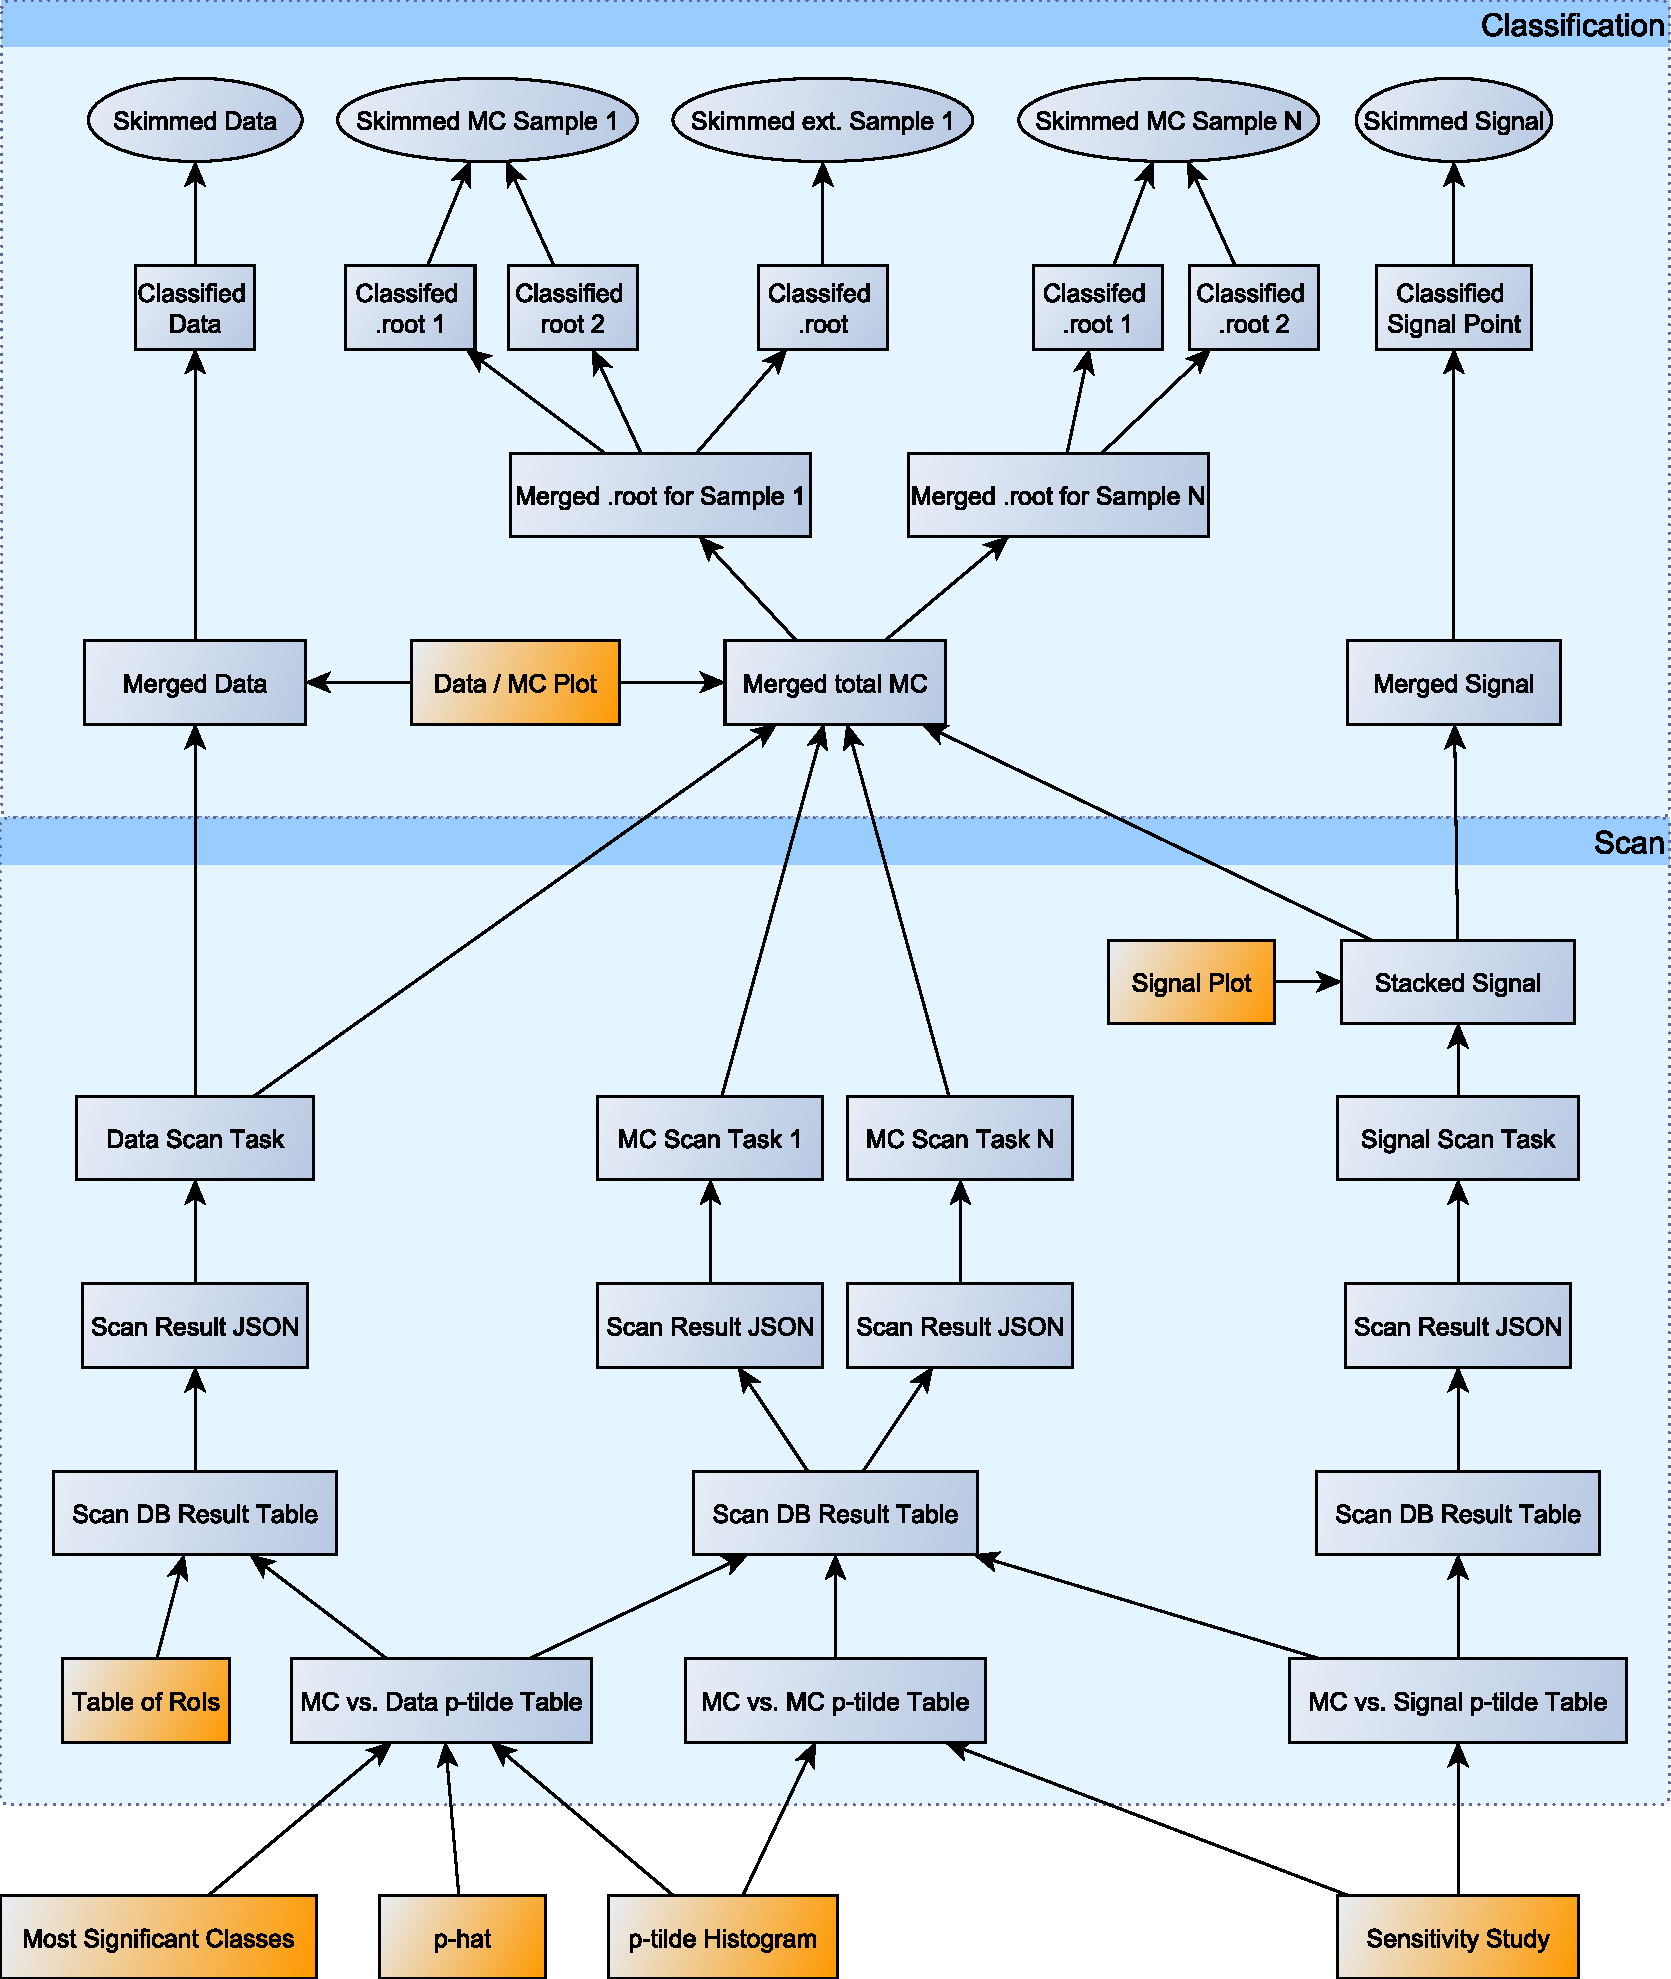
\includegraphics[width=\textwidth]{../music-workflow}
    \vspace{0.5em}
    \caption{Implementation of the MUSiC-Workflow. Using the Luigi-Automation Framework, these steps are performed on demand.}
    \label{fig:music_workflow}
\end{figure}


\subsection{Lookup-Table}
During the automated search algorithm, most of the computation time is spent calculating \TS according to \todo{ref?}, which involves integration and summation over a large number of terms.

To decrease the amount of time spent in this step, we implemented a three dimensional \acfi{LUT}. The table consists of \TS values for the most frequently used input parameters, such that the expensive runtime computation is replaced by retrieving a precomputed value from a static block of memory.

The \acf{LUT} is generated as a separate file during compilation and is about \SI{80}{\mega\byte} in size.

\subsubsection{Implementation}
The precise lookup procedure for $\TS_\text{LUT}(N_\text{obs}, N_\text{MC}, \sigma)$ \todo{parameter names and order?)} is as follows:
\begin{enumerate}
    \item Determine real-valued indices $i, j, k$ from the parameter values $N_\text{obs}, N_\text{MC}, \sigma$
    \item Check whether the calculated indices are valid, e.g. within table bounds
    \item Fetch four adjacent values from memory: $N_\text{obs}$ entry at $\floor i$, $N_\text{MC}$ and $\sigma$ entries at $\floor j, \ceil j, \floor k, \ceil k$.
    \item Use two dimensional linear interpolation in the $j, k$ plane to get a better estimate for \TS:
    \begin{align*}
        \TS_\text{LUT}(i, j, k) \approx \; &\TS(\floor i, \floor j, \floor k)(\ceil j - j)(\ceil k - k) \\
        + \; &\TS(\floor i, \ceil j, \floor k) (j - \floor j)(\ceil k - k) \\
        + \; &\TS(\floor i, \floor j, \ceil k) (\ceil j - j)(k - \floor k) \\
        + \; &\TS(\floor i, \ceil j, \ceil k) (j - \floor j)(k - \floor k)
    \end{align*}
    Note that $j - \floor j = 1 - (\ceil j - j)$.
    \item Discard the result if it is too small (less than $0.005$)
\end{enumerate}

If the value has not been found in the \ac{LUT}, either because of the table bounds or an otherwise untrusted value, the implementation falls back to the full expensive calculation of \TS.
Thus, the efficiency of the \ac{LUT} is determined by the probability that a requested value is contained in the table.

In order to improve accuracy around the most commonly used parameters ($N_\text{obs} = N_\text{exp}$, $N_\text{obs}$ small), the \ac{LUT} is organized in three regions, as illustrated in \fref{fig:lut_points}. In the so-called "grid region", the point spacing for the expected number of events is independent if the observed number of events. This results in a rectangular grid up to an observed yield of \num{10} and an expected yield of \num{20}.
The second, so-called "linear region" stretches up to an observed yield of \num{100}. In this region, every integer observed value corresponds to exactly one index, $i = N_\text{obs}$. Lastly, there is an exponential region, in which the spacing of observed points gradually becomes less dense, keeping the relative spacing constant.
In the dimension of the expected number of events, the \ac{LUT} is more densely spaced around $N_\text{exp} = N_\text{obs}$, because this is statistically the most common scenario. There is an exponential falloff in density which in theory expands from $N_\text{exp} = \num{0.1} N_\text{obs}$ up to $\num{5.0} N_\text{obs}$, very distant values, however, are vetoed by the $\TS_\text{LUT} > \num{0.005}$ threshold. In the third dimension, uncertainty, the grid is exponentially spaced in terms of relative uncertainty, from $\sigma = \num{0.01} N_\text{exp}$ up to $\num{2.0} N_\text{exp}$.

\subsubsection{Validation}

VALIDATION/COMPARISON TO FULL p:

Parameters determined to keep relative deviation from the "exact" p value below 1 percent

Comparison between computed p value and p from LUT for different values of rel. uncert in \fref{fig:lut_reldiff_reluncert} and for multiple values of data and MC in \fref{fig:lut_reldiff_mc}. Relative difference below dashed black line at 1 percent.

\begin{figure}
    \centering
    \includegraphics[width=0.7\textwidth]{lut/lut_points}
    \caption{LUT Points}
    \label{fig:lut_points}
\end{figure}

\begin{figure}
    \centering
    \includegraphics[width=0.49\textwidth]{lut/lut_uncert1}
    \includegraphics[width=0.49\textwidth]{lut/lut_uncert2}
    \caption{LUT Relative Differences depending on relative uncertainty}
    \label{fig:lut_reldiff_reluncert}
\end{figure}

\begin{figure}
    \centering
    \includegraphics[width=0.49\textwidth]{lut/lut0a}
    \includegraphics[width=0.49\textwidth]{lut/lut0b}
    \includegraphics[width=0.49\textwidth]{lut/lut1a}
    \includegraphics[width=0.49\textwidth]{lut/lut1b}
     \includegraphics[width=0.49\textwidth]{lut/lut2a}
    \includegraphics[width=0.49\textwidth]{lut/lut2b}
    \includegraphics[width=0.49\textwidth]{lut/lut3a}  
    \includegraphics[width=0.49\textwidth]{lut/lut3b}
    \caption{LUT Relative Differences depending on MC (fixed data)}
    \label{fig:lut_reldiff_mc}
\end{figure}

Additionally accessing coverage with lookup table
Same coverage result as for the full p value


